\chapter{Pixel detector geometry description\label{sec:matbudg}}

The CMS detector simulation uses an XML schema called the Detector Description Language (DDL) to encode the description of the detector geometry and material composition~\cite{CMS_AN_2005-000}. Together with two other auxiliary packages, the Algorithm Description Language (ADL) and Configuration Description Language (CDL), DDL interfaces with GEANT4 to provide the volumes, positions, and material compositions of the simulated detector elements.

All the various components and subcomponents of the CMS detector form a geometrical hierarchy, with each individual object being a subcomponent of some larger whole. In a system of XML files, DDL defines the basic data structures for describing the dimensions and materials of these parts as well as their geometrical hierarchies.

Two different classes of material definitions exist in DDL. Elementary materials correspond to elements of the periodic table and are identified by name, periodic table symbol, density, atomic number, and atomic weight. Definitions of composite materials are built by specifying their fractional composition in terms of elementary materials, or even other composite materials; the data structure allows one to customize the density associated with a particular composite material. The radiation length and hadronic interaction length of composite materials are calculated from the material definitions in the XML files; these parameters are needed ifor the modelling of particle interactions with detector components.

Detector parts are defined by their material, their shape, and their position in the detector. The various types of 3-dimensional shapes (such as rectangular boxes, trapezoids, and cylinders) allowed in this package are based on the GEANT syntax. Various parameters such as angles and Cartesian coordinates encode a detector component's spatial position, often with respect to a larger structure of which it is a component. Algorithms from ADL, referred to as DDAlgorithms, are used to position multiple copies of a detector component in a specific pattern, to represent symmetrical or repeating structures.

The rest of this chapter treats the projects involving the CMS pixel detector geometry description, in which I have participated.

\section{Pilot system simulation\label{sec:matbudg-pilot}}
%1. Pilot system simulation (mention of Phase I upgrade, LS1, installation of pilot system, how it was added to the description, figures)

From February 2013 to February 2015, the LHC was turned off. During this period of planned off-time, while the LHC was being prepared for proton-proton collisions at the design centre-of-mass energy $\sqrt{s} =$ 14 TeV, the CMS collaboration took the opportunity to perform repairs and maintenance on the CMS detector and install a new beampipe with a smaller diameter. To make room for the beampipe replacement, the pixel detector was extracted from the experimental cavern. While it was being stored in a lab aboveground, longstanding problems with its panels and electronics were diagnosed and fixed, and the barrel and endcap systems were calibrated in preparation for reinstallation in the cavern.

In addition to repairs and calibration, one extra endcap disk was installed on the -z side of the forward pixel detector (FPIX). 8 prototype modules for the planned Phase I upgrade~\cite{Dominguez:1481838} were mounted on the blades of this extra disk; Figure~\ref{fig:pilotmodules_actual} shows the third half-disk in one of the -z FPIX half-cylinders, with the Phase I prototype modules mounted. DC-DC converters and portcards were also installed in the service cylinder, to power the third disk and read out the modules respectively. Since this extra disk and its associated electronics serve as a pilot run for the Phase I modules, the ensemble is referred to as the pilot system.

\begin{figure}[hbtp]
  \begin{center}
    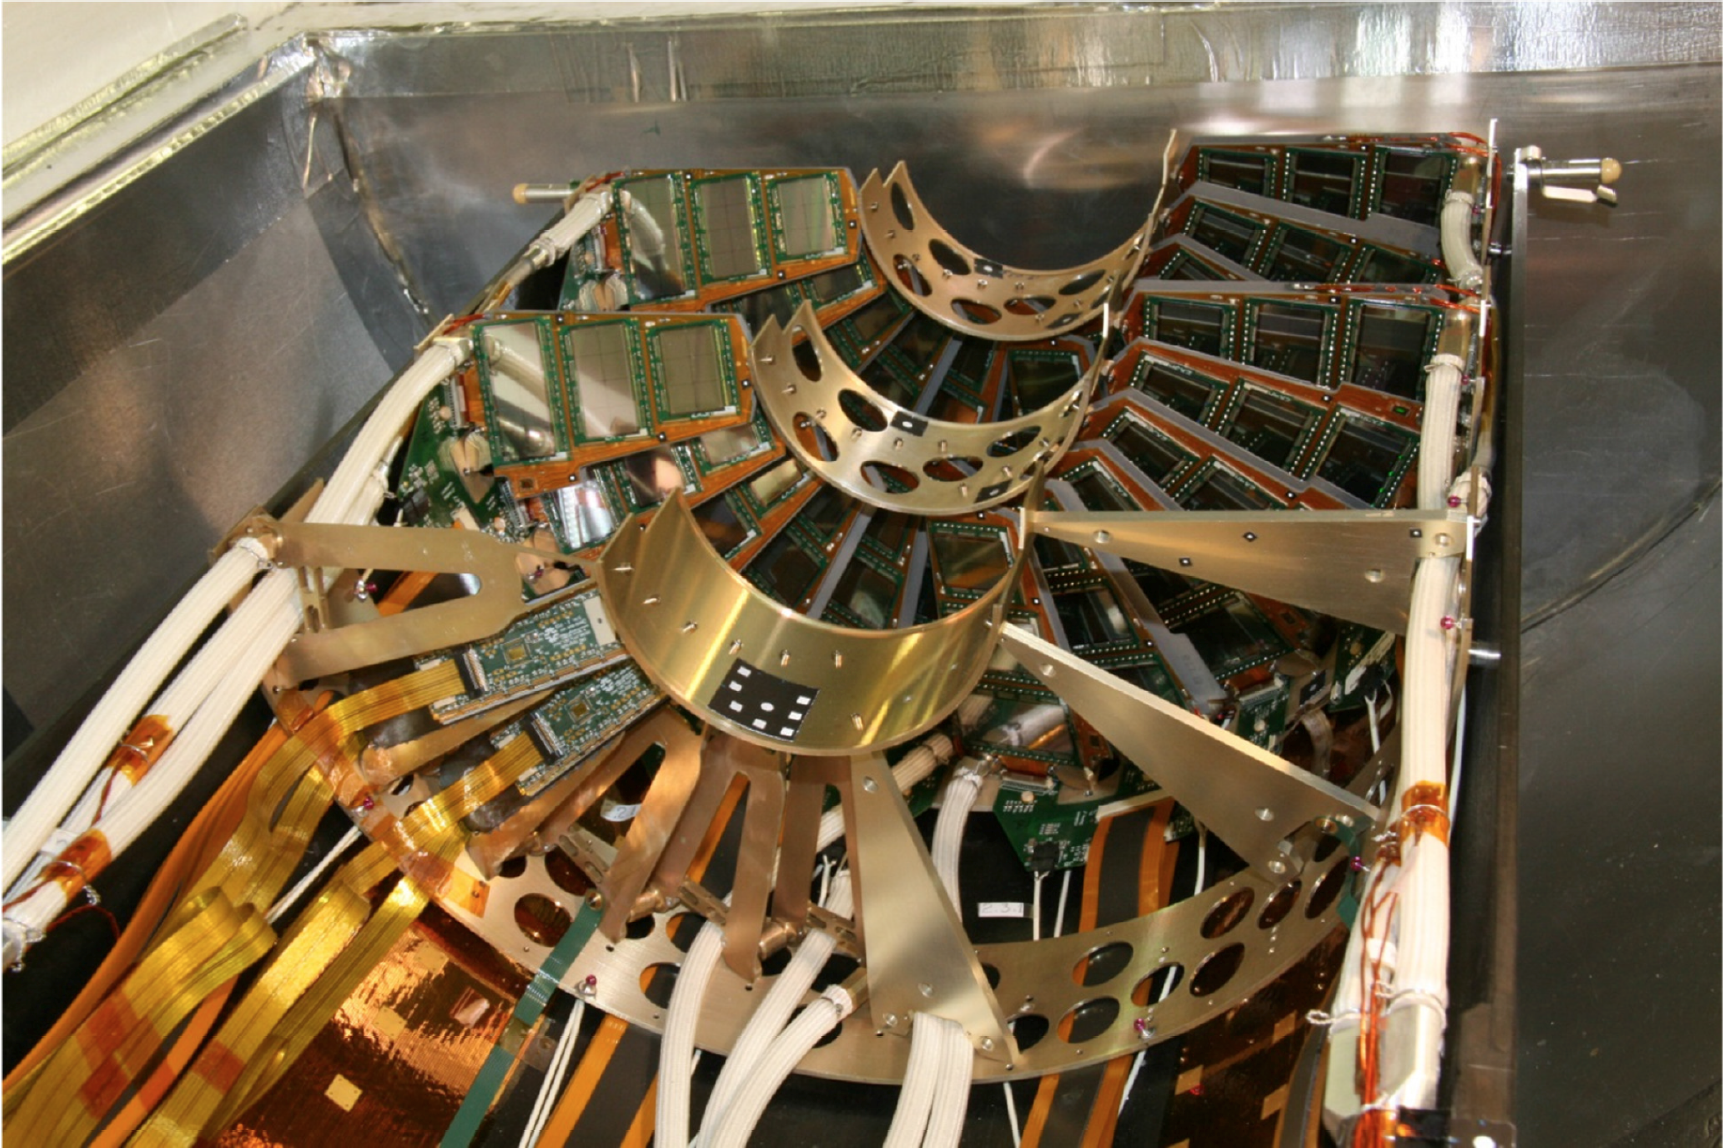
\includegraphics[width=\cmsFigWidth]{figures/Modules}
    \caption{-z FPIX half-cylinder, containing one pilot half-disk (foreground) in addition to its two standard half-disks.}
    \label{fig:pilotmodules_actual}
  \end{center}
\end{figure}

The tracker geometry and material description at the time did not include a description of the pilot system. In order to have an accurate representation of the material distribution (often referred to as the material budget) in the tracker for generating MC events with this new pixel detector configuration, the pilot system needed to be added to the description.

A disk on the -z endcap was cloned into the position where the new disk was installed; new objects were declared in the geometry description to represent the shape and material of the new modules. The large uniform blocks roughly representing the FPIX portcard electronics in the service cylinder also were updated, since the material composition had changed due to the addition of copper-containing DC-DC converters and other new electronics for the pilot system's readout. Thus, a new composite material representing the new average material composition was defined. Figure~\ref{fig:pilotmodules_sim} shows a visualization of the simulated pilot disk with its modules. Figure~\ref{fig:pilotelectronics} shows the configuration of FPIX service cylinder electronics prior to the pilot installation, as well as an illustration of the pilot system in the final simulation.

\begin{figure}[hbtp]
  \begin{center}
    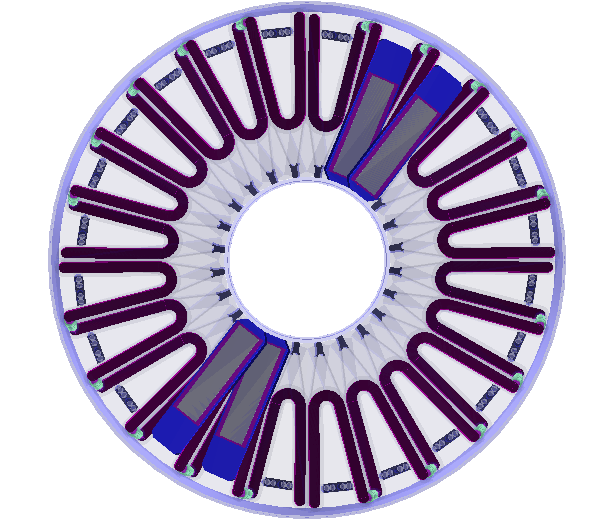
\includegraphics[width=\cmsFigWidth]{figures/ModulesCorrectedFurther}
    \caption{Fireworks visualization of the added pilot disk with its modules in the FPIX geometry description.}
    \label{fig:pilotmodules_sim}
  \end{center}
\end{figure}

\begin{figure}[hbtp]
  \begin{center}
    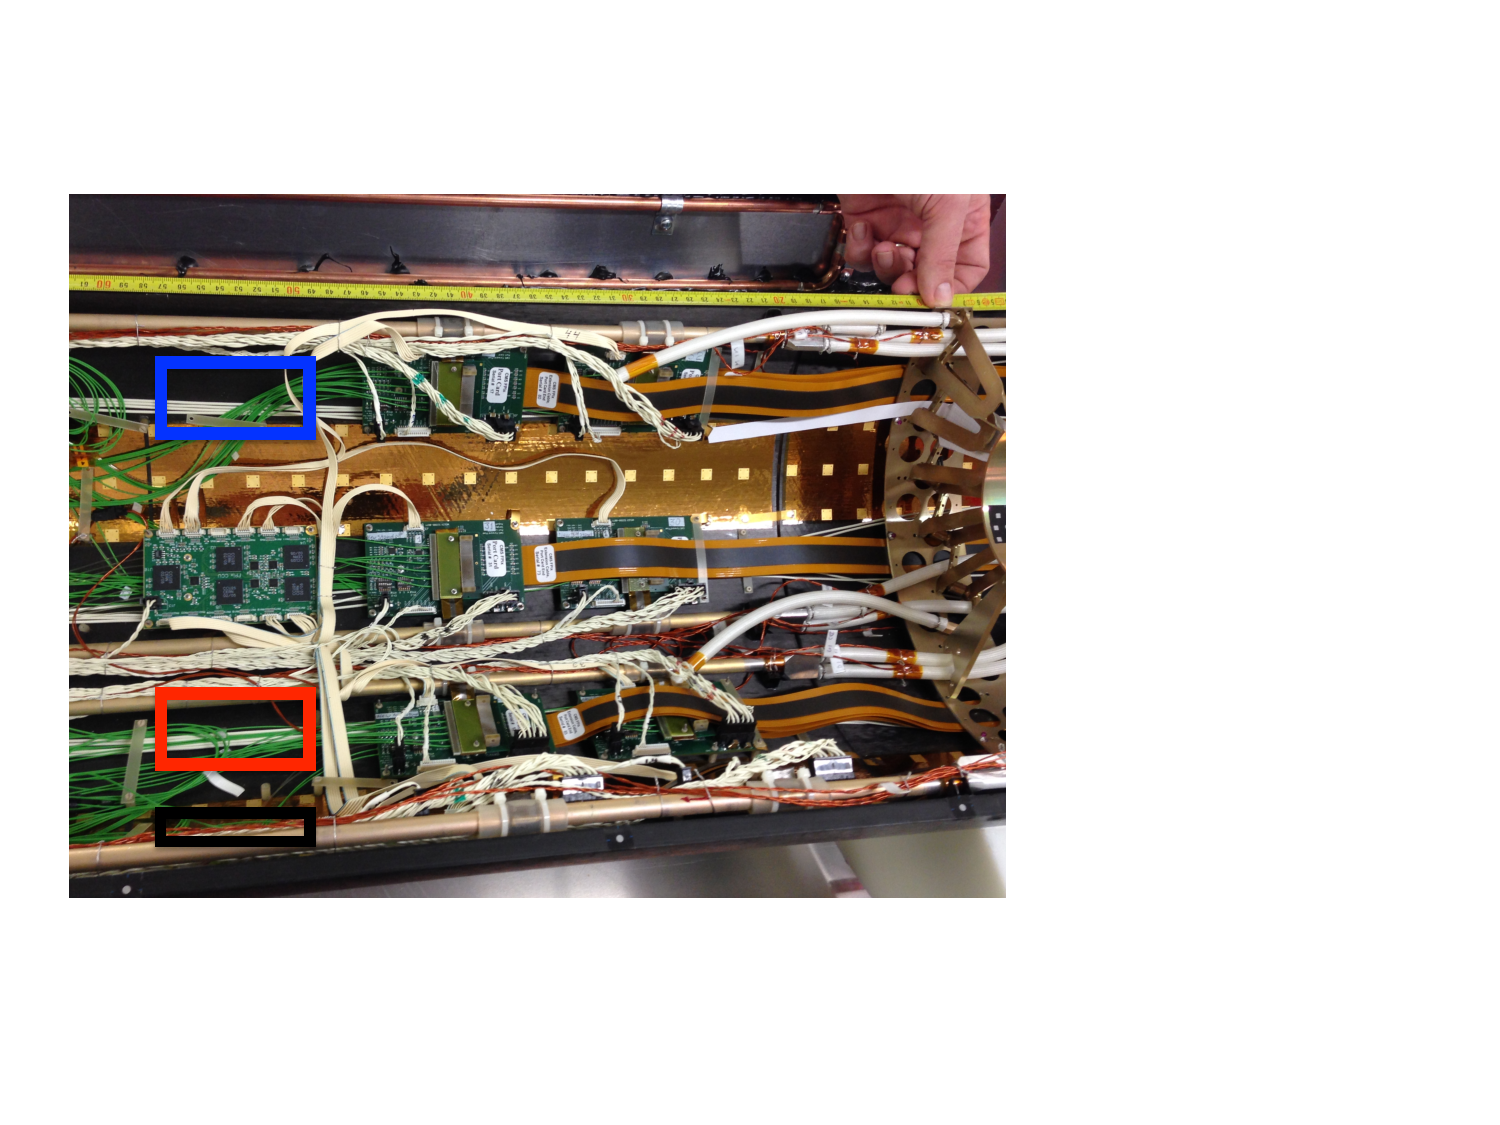
\includegraphics[width=1.24\cmsFigWidth]{figures/pilotelectronics_actual}
    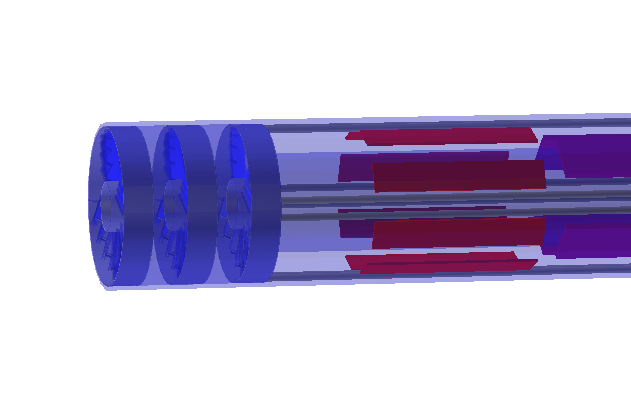
\includegraphics[width=1.24\cmsFigWidth]{figures/PilotGeom_8PortCards2}
    \caption{(\cmsLeft) The FPIX service cylinder before the pilot system installation. The rightmost two columns of circuitboards are the portcards for the two standard FPIX half-disks. The leftmost column contains only the digital communication and control unit (CCU) for the two FPIX half-disks. The coloured rectangles indicate the intended positions of the pilot electronics to be installed. Red: CCU board. Blue: Portcard. Black: DC-DC converter board. (\cmsRight) Fireworks visualization of the pilot system in the FPIX geometry description. The pilot disk is the third from the left, and the red rectangles represent the portcard electronics in the service cylinder.}
    \label{fig:pilotelectronics}
  \end{center}
\end{figure}


\section{Phase I pixel geometry simulation\label{sec:matbudg-phase1}}
%2. Updates to Phase I description (ongoing; mostly done, describe what is being corrected)

During the next long shutdown of the LHC scheduled for 2018, the CMS detector will undergo another round of detector upgrades referred to as the Phase I upgrade~\cite{Dominguez:1481838}, to fix weaknesses in the current systems and improve detector performance at the higher luminosities expected in the future. The pixel detector will acquire one new barrel layer and one new endcap on each side of the interaction point, to provide redundancy in track hit pattern recognition, reduce fake rates at high pileup, and still allow decent tracking performance even if the inner layer undergoes more radiation damage than expected. Faster electronics will be installed, for efficient operation at high event rates. The cooling system, which currently uses C$_{6}$F$_{14}$ as a coolant, will be replaced with a more lightweight cooling system that uses cold carbon dioxide instead. In general, the design of the upgraded pixel detector's support structures is aimed at decreasing the material budget in the tracking volume.

The CMS geometry description currently has XML files that describe the Phase I pixel geometry and material. The barrel pixel part is mostly accurate aside from a few minor changes involving the dimensions of some support structures and the addition of aluminium cabling in some regions. However, the forward pixel part is very inaccurate and needs significant updating in order to represent the actual upgraded components that will be installed. The main challenges are the following:

\begin{itemize}
\item The current description of the FPIX support rings are flat, uniform rings, whereas the actual support rings have a zigzagging shape (see Figure~\ref{fig:phaseI_diskcomparison}). This is extremely difficult to render using the shapes allowed in DDL. A tentative solution is being developed and tested, in which a series of ``infinitesimally" thin blocks are positioned in the form of a zigzag-shaped ring using a DDAlgorithm that gives each block an appropriate displacement along z as a function of $\phi$. Figure~\ref{fig:phaseI_disksolution} illustrates this proposed solution.
\item The zigzag pattern of the blades in the rings is incorrect for some of the rings, as they do not have the proper symmetry about the y axis. Comparisons with the blueprints of the actual Phase I FPIX blades in their disks are currently underway to determine the correct symmetry.
\item In simulation, the endcap disks on the +z side are obtained by rotating the -z disks about the y axis, whereas the actual Phase I disks have a mirror symmetry about the xy plane instead.
\item The shapes of the modules and the blades need to be refined, as they currently have very rough and basic shapes in the simulation (see Figure~\ref{fig:phaseI_bladecomparison}).
\item The composite material used to describe the Phase I portcard objects is the same material used to describe the portcard objects in the Run I geometry before the installation of the pilot system. This is clearly incorrect, and a new composite material needs to be declared that matches the average composition of the actual Phase I FPIX portcards and DC-DC converters.
\end{itemize}

Since January 2015 and continuing into my postdoctoral position, I have been the convener of the CMS tracker material budget group, overseeing any tasks that involve changes to the geometry/material description or studies of the tracker structure in data. I have contributed most directly to updating the Phase I pixel geometry description, and much of this work is still ongoing. In particular, I designed the proposed solution for representing the zigzag-shaped FPIX support rings, which is still being tested and refined. I am communicating with the engineers who are building the Phase I FPIX and BPIX components, to get the necessary information about their dimensions and material composition to represent them accurately in the simulated description.

Also, I am overseeing a group that is updating a code package for reconstructing and analyzing nuclear interaction vertices, so as to be able to use reconstructed nuclear interaction vertices in the tracker material to image the structure of the tracker, measure the positions of tracker structures and the beam-pipe, and validate the geometry description in simulation. My contribution consists of providing technical support for dealing with the simulated geometry description.

\begin{figure}[hbtp]
  \begin{center}
    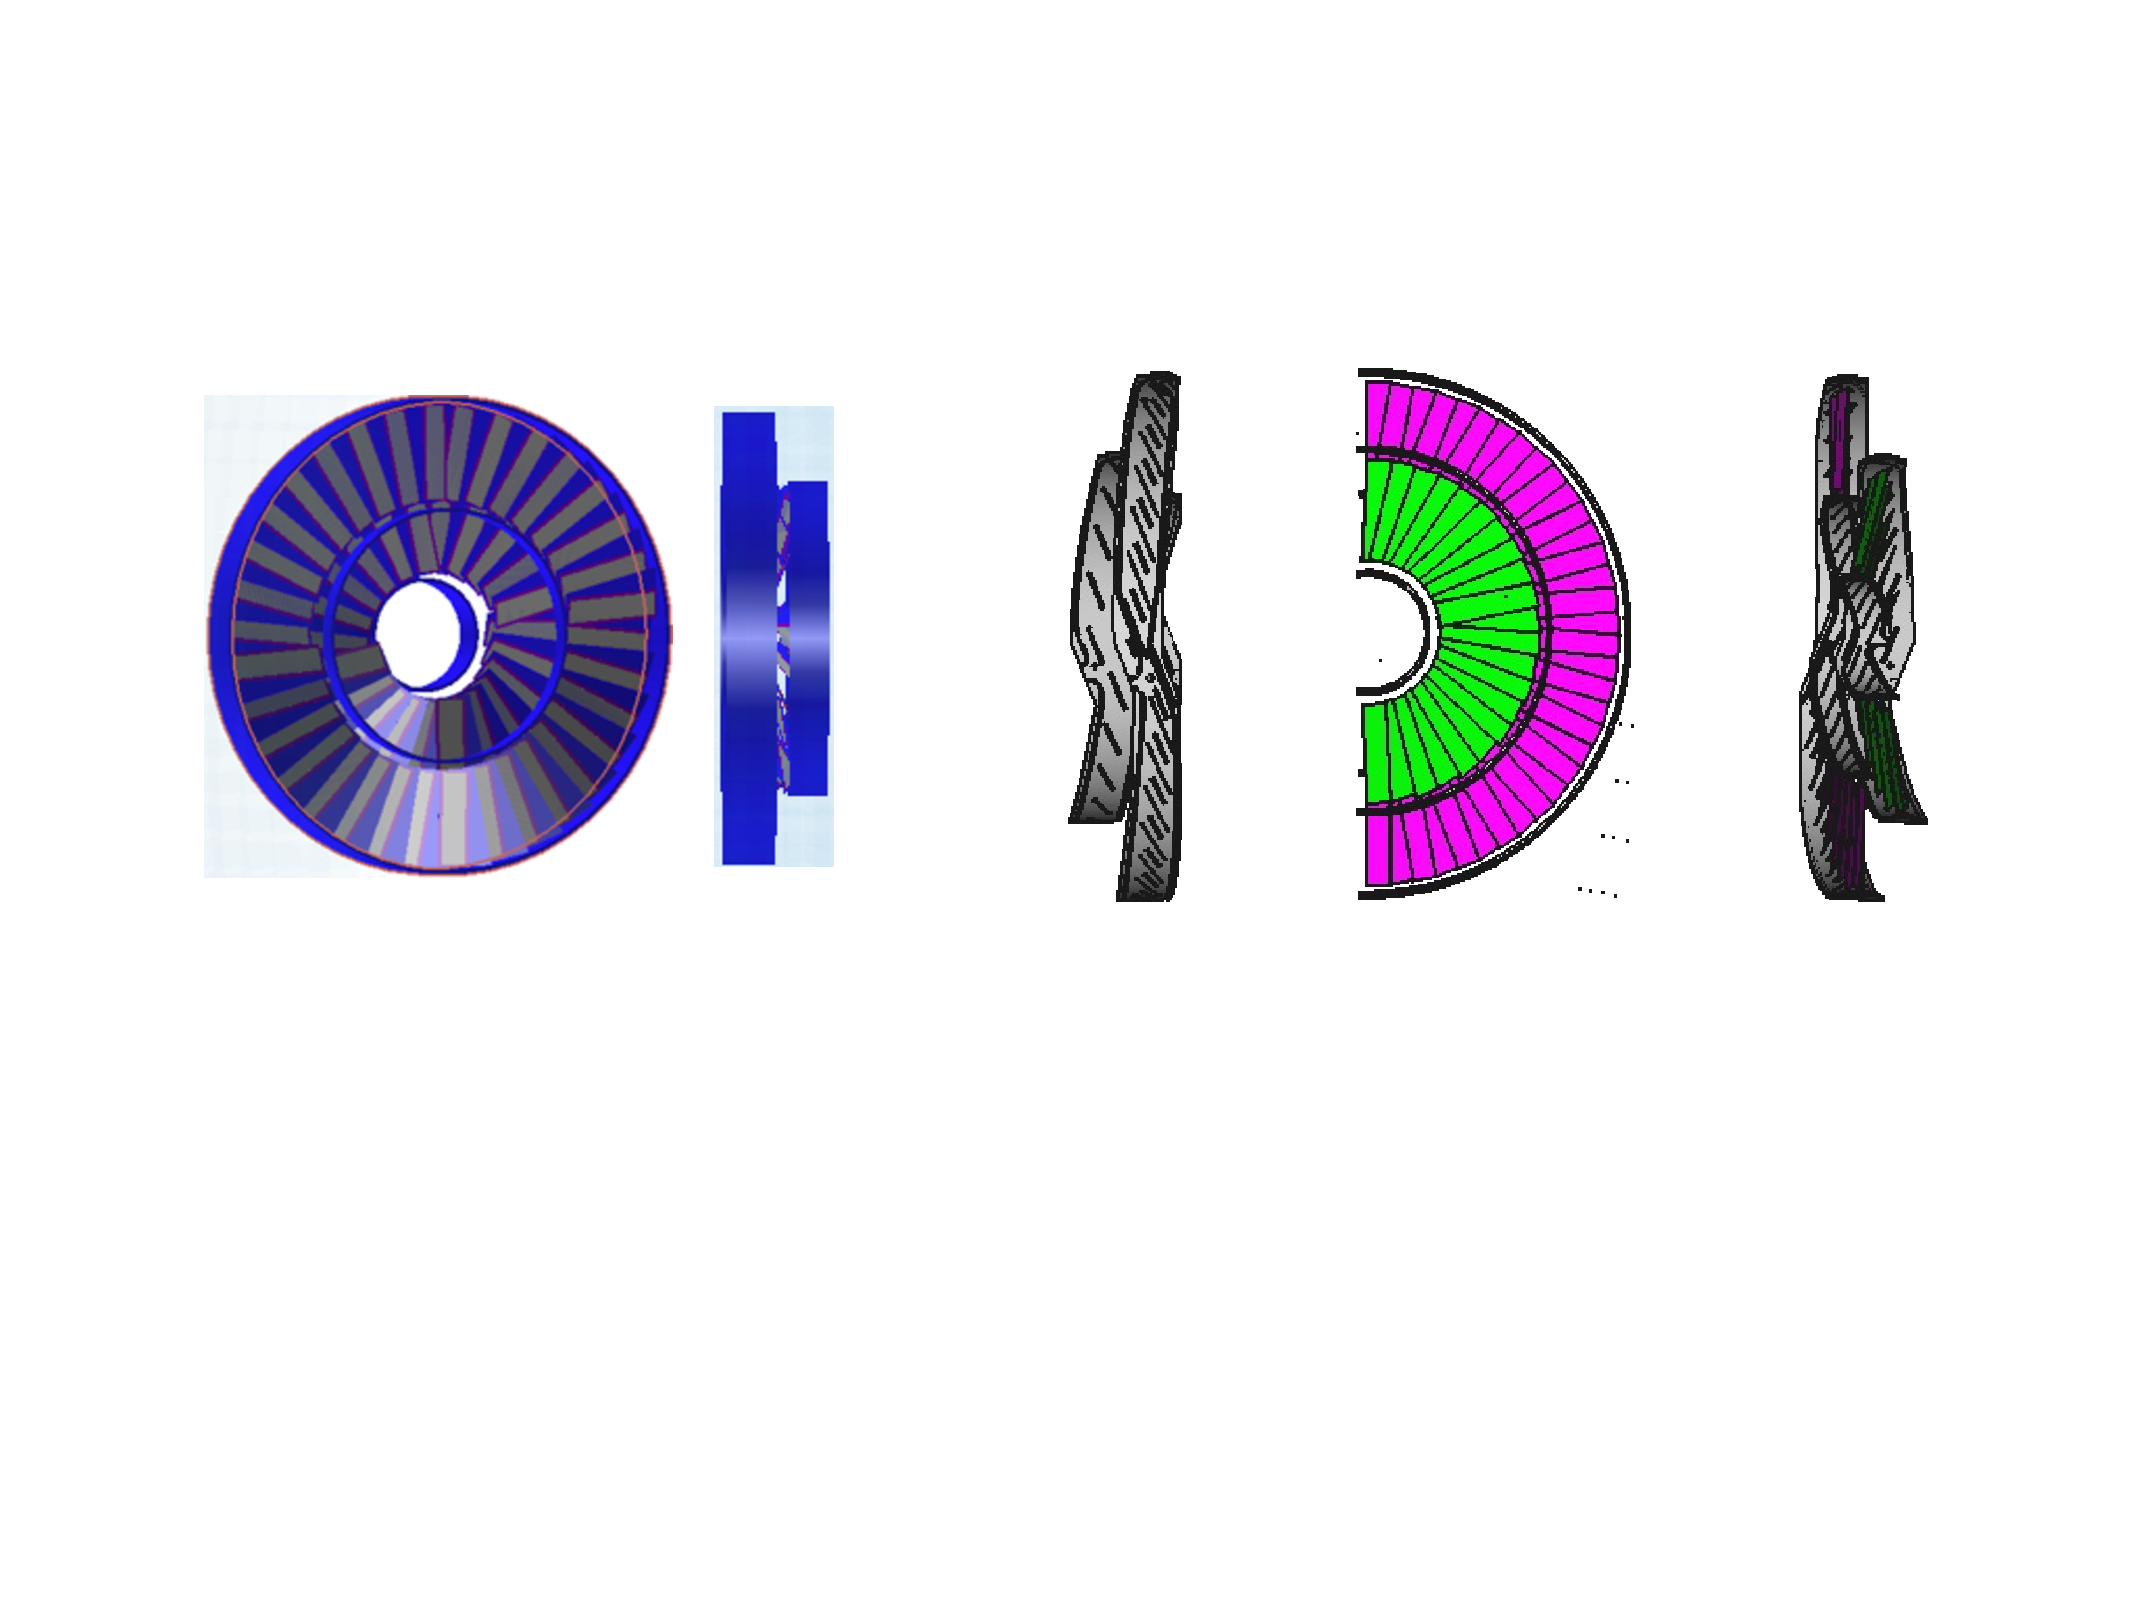
\includegraphics[width=2.0\cmsFigWidth]{figures/phaseI_diskcomparison}
    \caption{Comparison of the shape of the Phase I FPIX half-disks in simulation (\cmsLeft) and in the actual detector being constructed (\cmsRight).}
    \label{fig:phaseI_diskcomparison}
  \end{center}
\end{figure}

\begin{figure}[hbtp]
  \begin{center}
    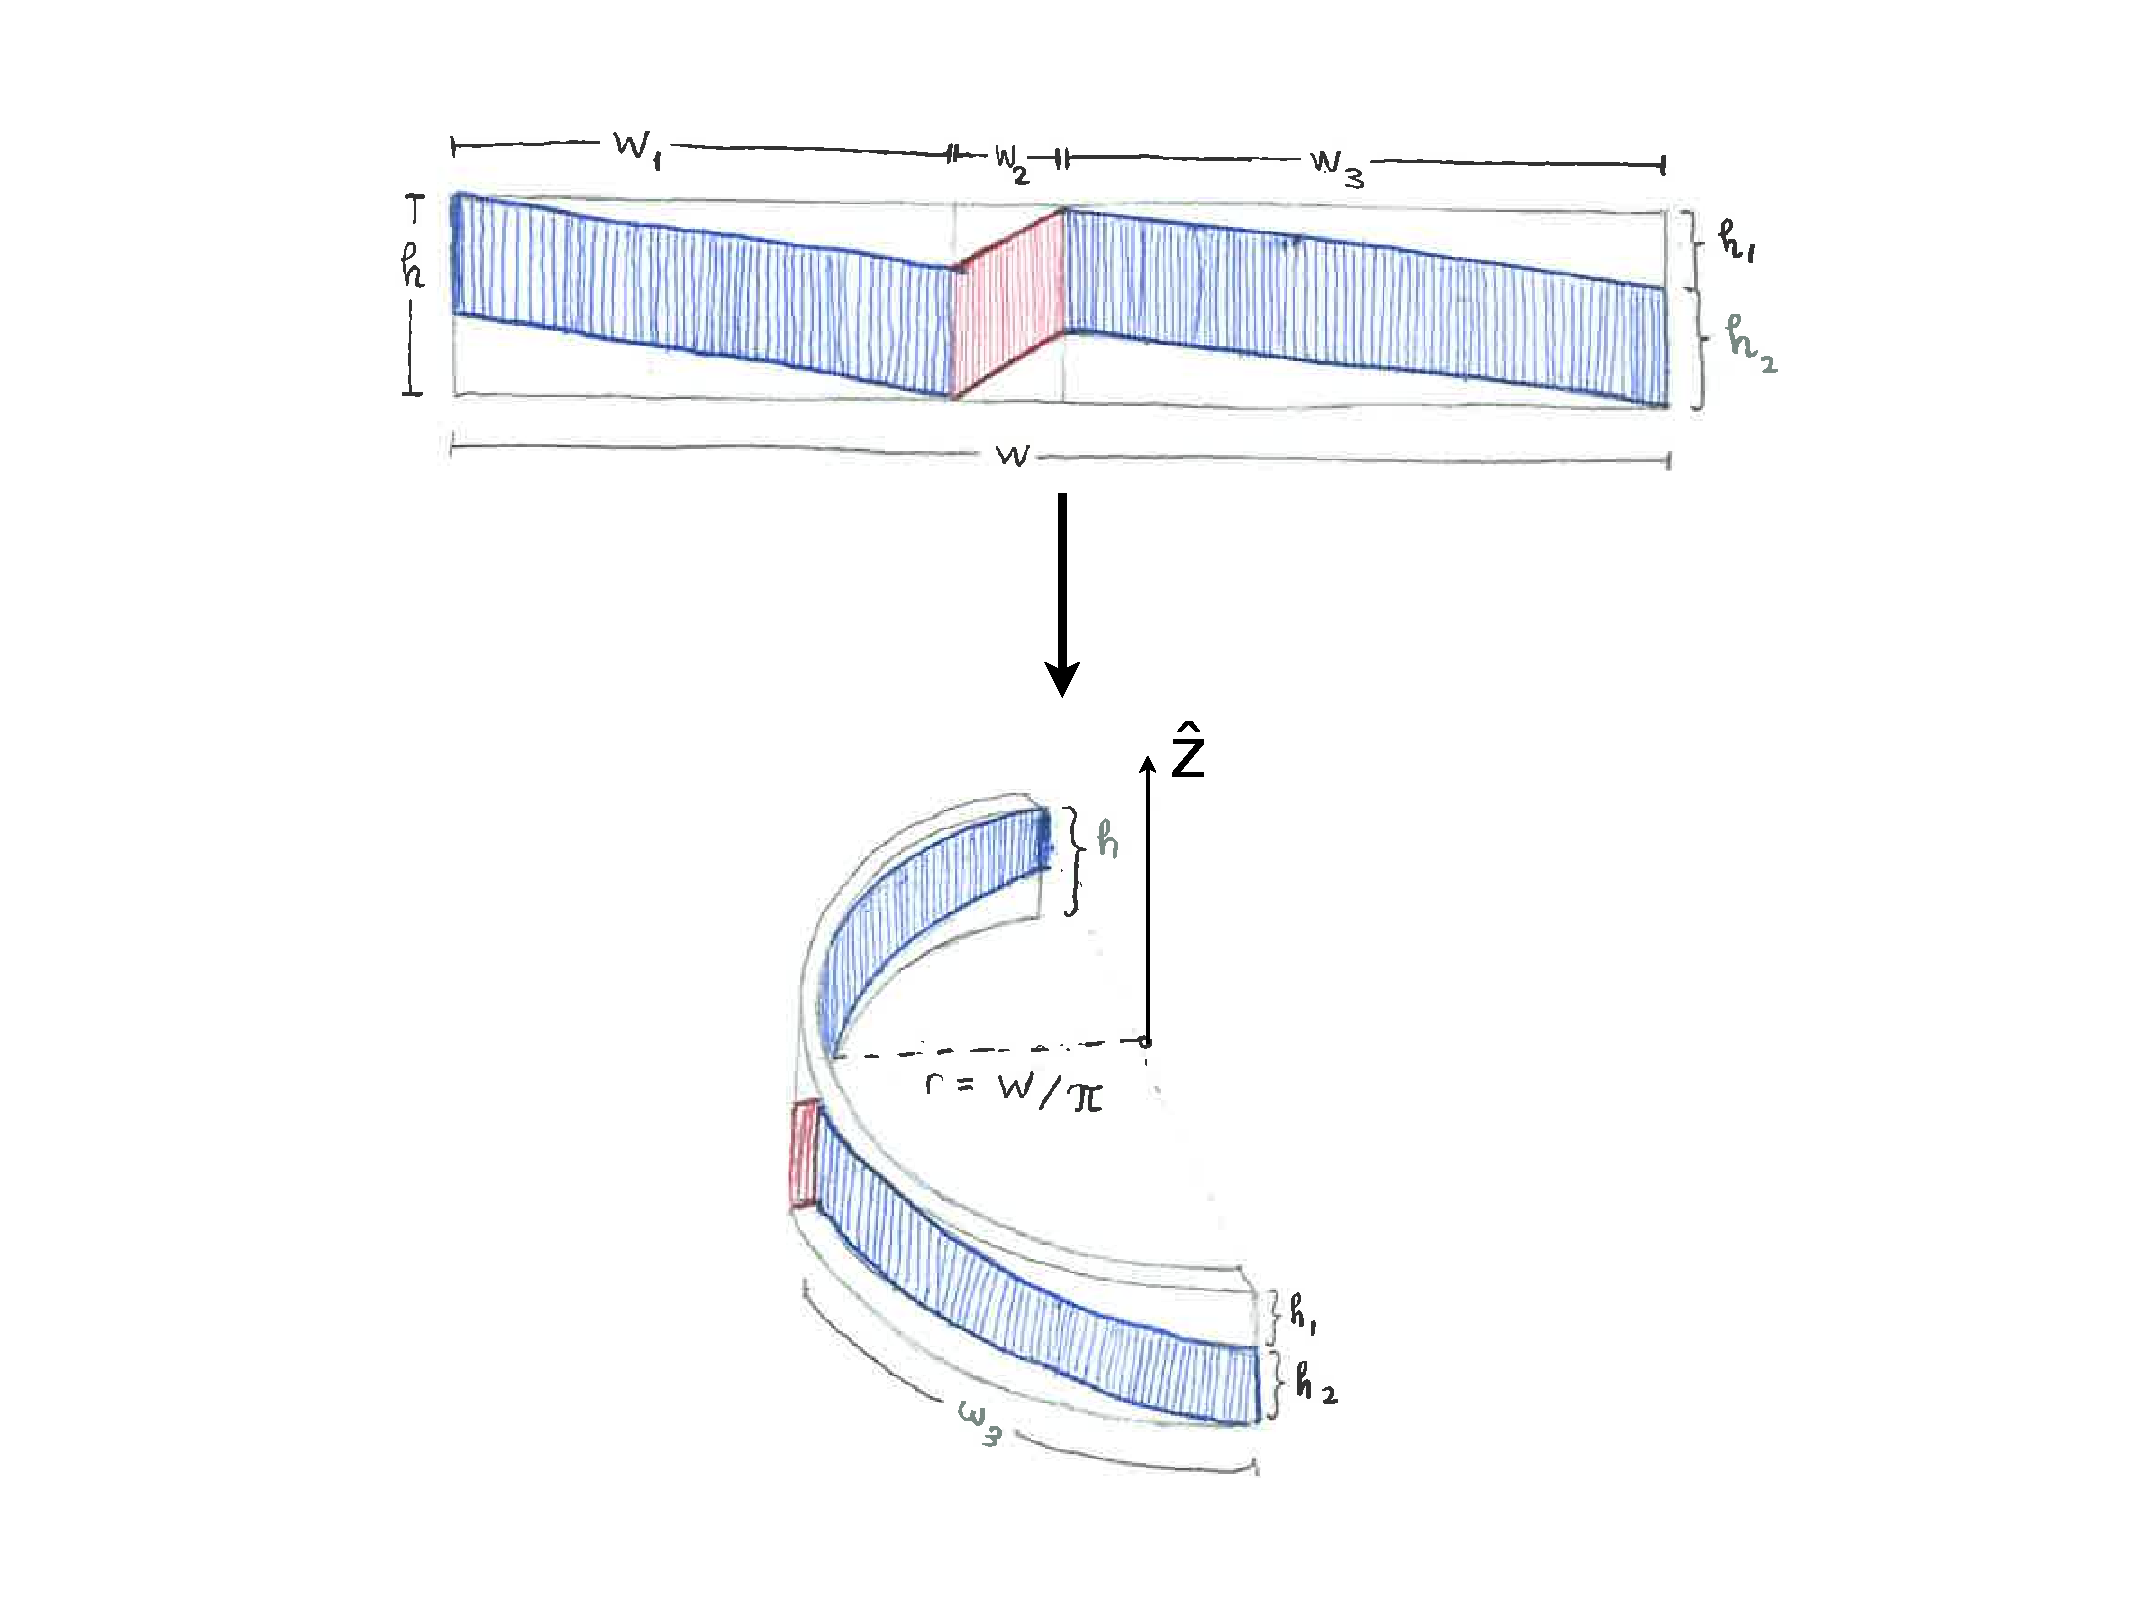
\includegraphics[width=2.0\cmsFigWidth]{figures/phaseI_disksolution}
    \caption{Illustration of the proposed solution for modelling the zigzag-shaped support rings of the Phase I FPIX half-disks. The blue and red colours denote the three basic legs that make up the zigzag. A DDAlgorithm is used to position thin rectangular blocks into an approximation of the zigzagging shape by arranging them in a ring and giving each block an incremental displacement in the z-direction from the plane of the ring, where the displacement depends on the azimuthal angle $\phi$ around the ring.}
    \label{fig:phaseI_disksolution}
  \end{center}
\end{figure}

\begin{figure}[hbtp]
  \begin{center}
    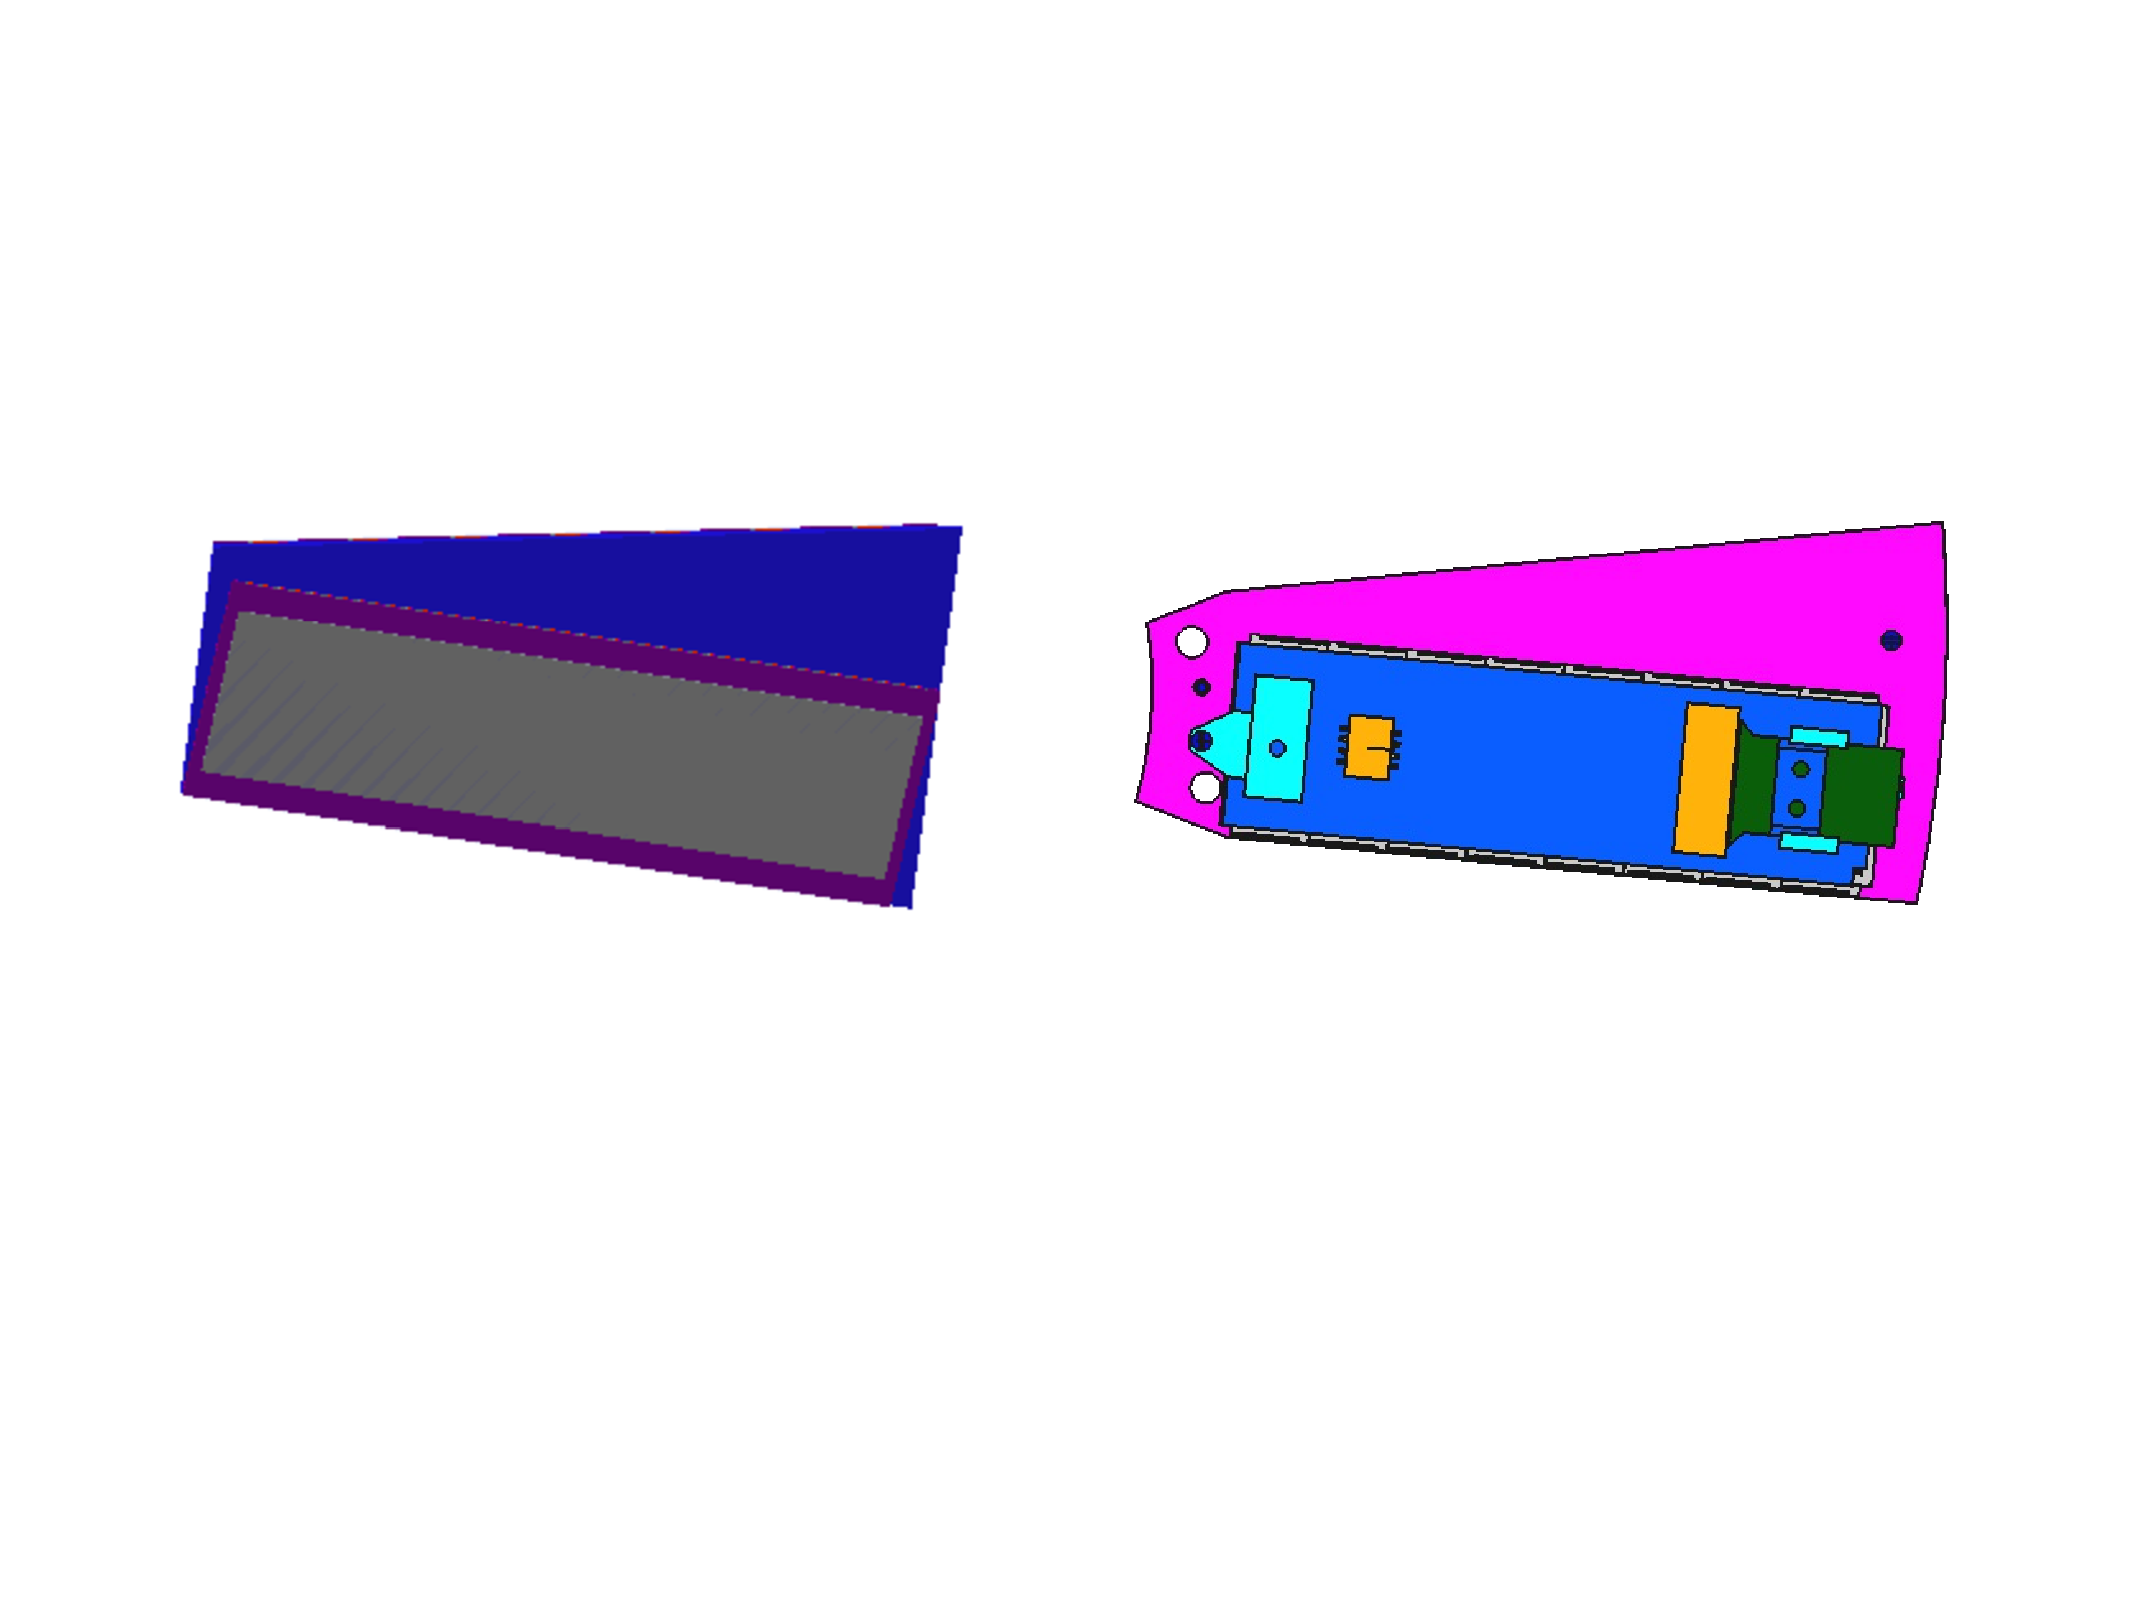
\includegraphics[width=2.0\cmsFigWidth]{figures/phaseI_bladecomparison}
    \caption{Comparison of the shape of the Phase I FPIX blades and modules in simulation (\cmsLeft) and in the actual detector being constructed (\cmsRight).}
    \label{fig:phaseI_bladecomparison}
  \end{center}
\end{figure}
